\documentclass{article}
\usepackage{amsmath, amssymb, amsthm}
\usepackage[UTF8]{ctex}
\usepackage{graphicx}
\usepackage{subfigure}
\usepackage{float}
\usepackage{geometry}
\usepackage{fancyhdr}
\usepackage{hyperref}
\usepackage{siunitx}
\usepackage{tikz}
\usepackage{fontspec}
\usepackage{epsfig}
\fontspec{Times New Roman}
\usepackage{enumitem}
\geometry{a4paper, scale=0.8}
\usetikzlibrary{arrows,shapes,automata,petri,positioning,calc,shapes.geometric}
\usetikzlibrary{decorations.pathreplacing, decorations.markings}
\tikzstyle{spring}=[thick,decorate,decoration={zigzag,pre length=0.1cm,post
  length=0.1cm,segment length=6}]

\newcommand{\keywords}[1]{\textbf{关键词} #1}

\title{``魔板'' 加持下的平抛运动定理验证实验}
\author{吴承宇\ 20230616 \thanks{Ethan Goh (\texttt{<7086cmd@gmail.com>}). 本文的主要撰写者, 同时承担数据分析, 软件配置操作.} \and 陈麒泽\ 20231204 \thanks{基本上贡献相等. 搭建了实验模型, 参与了实验设计和文章撰写.} \and 胡铭轩\ 20231207 \footnotemark[2] \and 卢柯忻\ 20230534 \footnotemark[2] \and 张函毓\ 20231237 \footnotemark[2] \and 章嘉乐\ 20231226 \footnotemark[2]}
\date{\today}

\begin{document}

\maketitle

\abstract{
    通过朗威 (DISLab) 的 ``魔板'' 系统, 可以即时获取平抛物体的运动轨迹. 通过以时间, $x$ 轴坐标和 $y$ 轴坐标为变量的数据, 可以验证平抛运动的各项定理. 本实验通过 ``魔板'' 系统, 以及 ``魔板'' 系统配套的实验仪器, 验证了平抛运动的各项定理.

    在中学课本中, 平抛运动的定理的验证是通过复写纸, 通过速度的分解来分别得出数值和平行方向的运动特点, 进而验证平抛运动的模型. 然而, 传统实验中, 初始抛出小球的斜面需要人用手来控制小球的释放, 这可能导致一系列的系统误差.

    通过信息技术, 本组成员方便的获取了每 \qty{0.02}{\second} 的实验数据, 以通过回归的方式训练出描述轨迹的回归方程, 以验证平抛运动的定律.
}

\keywords{平抛运动; 实验改进; DISLab ``魔板''实验; 回归模型; 验证实验}

\tableofcontents

\section{问题分析}

对于平抛运动的轨迹, 理论上可以通过受力分析进行:

\begin{figure}[H]
    \flushright
    \begin{tikzpicture}[scale=0.8]
        \draw (0, 0) rectangle (4, 2);
        \draw[-latex] (2, 1) -- (2, -1) node[below] {$mg$};
    \end{tikzpicture}
\end{figure}

因此, 在水平方向上, 不计空气阻力则有 $F_x = 0$, 在竖直方向上, 有 $F_y = -mg$. 由牛顿第二定律, 可以得到:

\begin{equation}
    \begin{cases}
        a_{\perp} = -g \\
        a_{\parallel} = 0
    \end{cases}
\end{equation}

因此, 对其进行积分, 可以得到:

\begin{equation}
    \begin{cases}
        v_{\perp} = -gt + v_{0\perp} \\
        v_{\parallel} = v_{0\parallel}
    \end{cases}
\end{equation}

因此, 可以得到平抛运动的轨迹方程:

\begin{equation}
    \begin{cases}
        x = v_{0\parallel}t \\
        y = v_{0\perp}t - \frac{1}{2}gt^2
    \end{cases}
\end{equation}

因此, 可以通过实验验证平抛运动的定理.

\section{实验准备}

本实验通过朗威 (DISLab) 的 ``魔板'' (Magic Board) 系统进行实验. ``魔板'' 系统通过提供一个较大的竖直平台, 可以快速以 \qty{50}{\hertz} 等频率记录运动块的方位, 通过绘制散点图, 线型图等方式可以得到运动块的运动轨迹.

魔板系统可以视为一个抛出器与位置传感器, 整体如图 \ref{fig:magic-board} 所示.

\begin{figure}[H]
    \centering
    \begin{tikzpicture}[scale=0.8]
        \draw[help lines] (0, 0) grid (8, 6);
        \draw[->] (0, 6) -- (10, 6) node [right] {$x$};
        \draw[->] (0, 6) -- (0, -1) node [below] {$y$};
        \draw[dashed] (-4, 6) -- (-2, 6);
        \draw (-4, 5) rectangle ++(5, 2);
        \draw (1, 6) parabola bend (1, 6) (8, 0);
    \end{tikzpicture}
    \caption{``魔板'' 示意图}
    \label{fig:magic-board}
\end{figure}

\section{实验步骤}

本次实验设计步骤如下:

\begin{enumerate}
    \item 组装 ``魔板'' 系统, 并连接至电脑.
    \item 在计算机中打开 ``魔板'' 对应软件, 并将运动快放到抛出原点.
    \item 按照 $3$ 级弹簧压缩量, 以及 \ang{0} 的角度多次抛出是运动块.
    \item 导出实验数据, 通过 \texttt{scikit-learn} 库进行回归模型的分析, 并总结模型.
\end{enumerate}

该软件的界面如图 \ref{fig:software} 所示.

\begin{figure}[H]
    \centering
    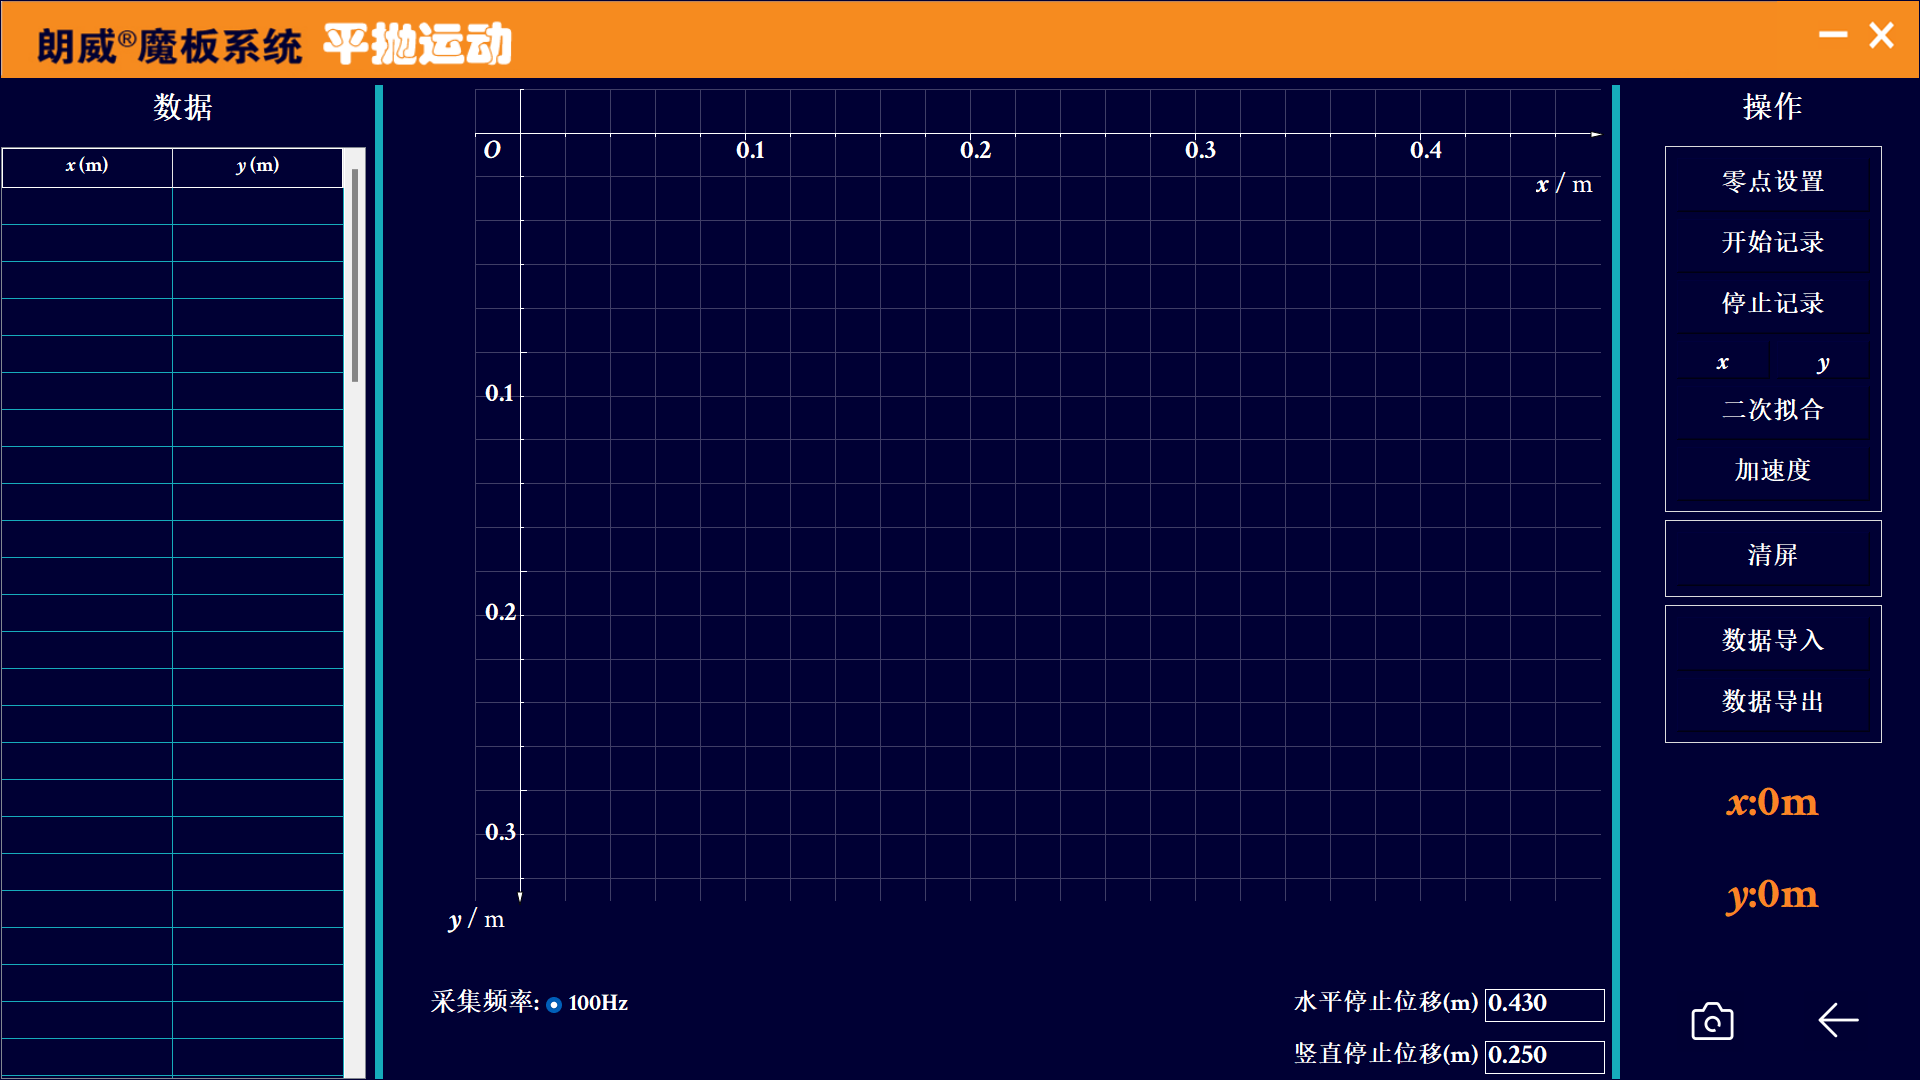
\includegraphics[width=0.6\textwidth]{figures/magic-board.png}
    \caption{``魔板'' 软件界面}
    \label{fig:software}
\end{figure}

通过多次实验, 笔者获得了 $4$ 组数据, 并保存在 \texttt{data} 文件夹中.

\section{实验数据分析}

以 \texttt{2024-05-17(16-57-14).csv} 中的数据为例, 通过 \texttt{matplotlib} 库, 笔者绘制出如下散点图:

\begin{figure}[H]
    \centering
    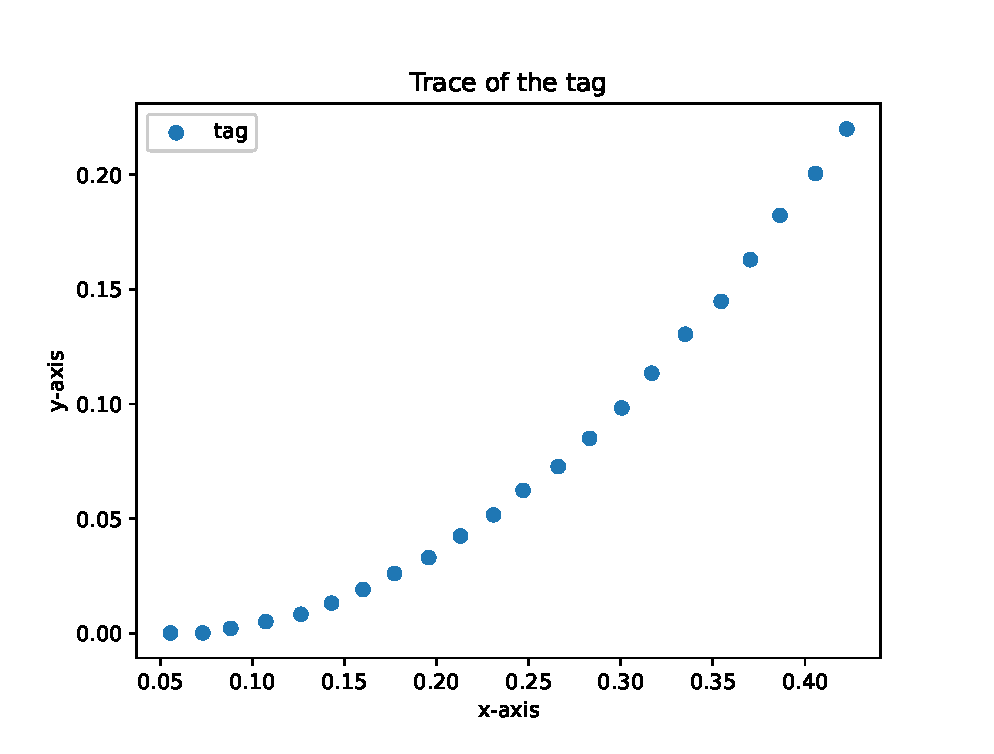
\includegraphics[width=0.6\textwidth]{figures/plot1.eps}
\end{figure}

因此, 我们对于所有的数据进行绘制, 得到如下的散点图:

\begin{figure}[H]
    \centering
    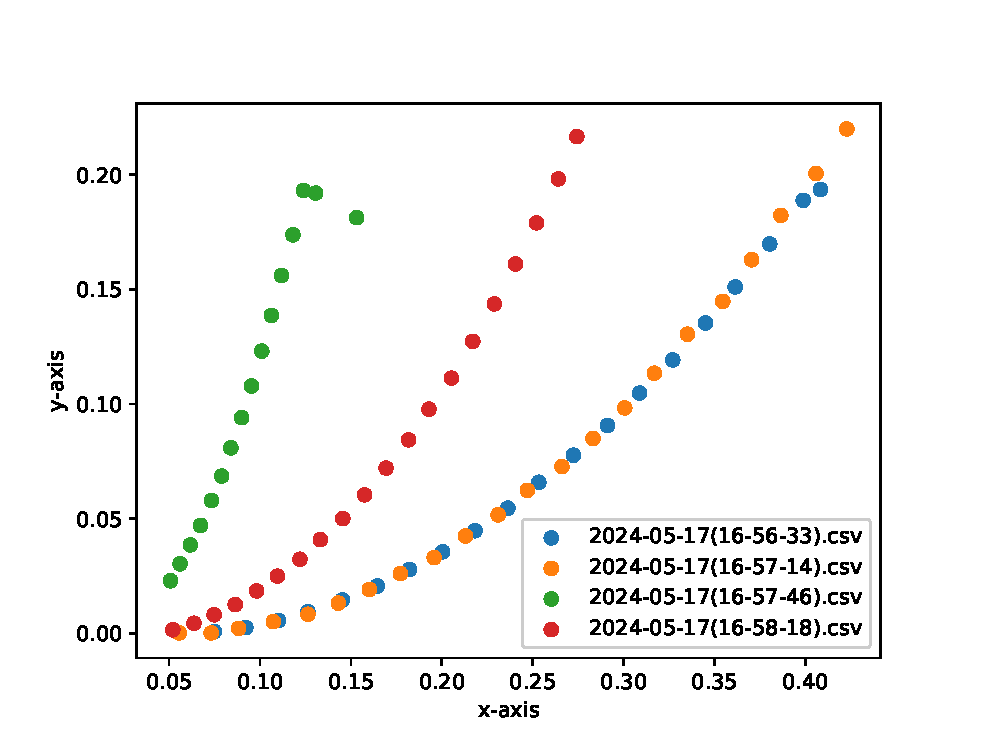
\includegraphics[width=0.6\textwidth]{figures/plot-all.eps}
\end{figure}

通过散点图的绘制, 发现实验数据 \texttt{2024-05-17(16-56-33).csv}, \texttt{2024-05-17(16-57-14).csv} 和 \texttt{2024-05-17(16-58-18).csv} 两份数据较有准确性, 因此采用这两组数据进行线性回归拟合来进行数据分析.

因此, 笔者通过 \texttt{scikit-learn} 的 \texttt{LinearRegression} 模型分别对于 $x - t$ (水平方向) 和 $y - t$ (竖直方向) 进行回归分析.

\end{document}
